\documentclass{article}
\input{/DocHeader.tex}
\title{Summary of methods for level set evolution by radius
  of curvature}
\author{By: Aaron Berk\\Supervised by: Dr. Nicholas
  Kevlahan\\McMaster University}
\date{Summer 2013}
\begin{document}

%%----------------------
% title page

\begin{titlepage}
\phantom{asdf.}

\vskip100pt
  \begin{center}
\rule{.85\textwidth}{1pt}\\[0.2in]
    {\huge \bfseries The evoLS library}\\[0.1in]
\rule{.6\textwidth}{.5pt}\\[0.1in]
    {\LARGE Documentation for the implementation of level set\\
      evolution by (generalized) radius of curvature}\\[0.1in]
\rule{.85\textwidth}{1pt}\\[1in]
\begin{minipage}{0.4\textwidth}
  \begin{flushleft}\large
    \emph{Author:}

Aaron \textsc{Berk}
  \end{flushleft}
\end{minipage}
\begin{minipage}{0.4\textwidth}
  \begin{flushright}\large
    \emph{Supervisor:}

Dr. Nicholas \textsc{Kevlahan}
  \end{flushright}
\end{minipage}

\vfill

\begin{minipage}{0.5\textwidth}
  \begin{center}\large
    Department of Mathematics \& Statistics

\textsc{McMaster University}
  \end{center}
\end{minipage}

\vfill
{\large \today}
  \end{center}
\end{titlepage}

% /title page
%%---------------------------

\section{Introduction}
\label{sec:introduction}

Each of the number of tsunamis that have occurred in the recent
past has demonstrated the awesome amount of destruction of which
these natural disasters are capable. The ability to use realistic
numerical simulations to understand better the myriad factors
affecting tidal flow could help in the design of effective
countermeasures against tsunamis. However, the construction of a
realistic numerical simulation is entirely non-trivial. Several
tools are required to construct such a simulation of tidal flow on
the surface of the Earth (\ie tidal flow subject to realistic
bottom bathymetry and coastline data). The method will be based on
solving an incarnation of the shallow water equations using an
adaptive wavelet collocation scheme, with boundary conditions
implemented via Brinkman penalization (refer to \cite{reckinger}
for a more thorough summary of these methods).

Subject to the methods mentioned above, working with realistic
bottom bathymetry and coastline data of the Earth is another
non-trivial aspect of constructing a realistic numerical
simulation. Because of the ability of adaptive wavelet methods to
``zoom in'' on regions of the domain that require higher resolution,
it is necessary to be able to control how finely, how accurately
and how smoothly the coastline can be discretized at arbitrary
regions throughout the grid. When fine scale features must be
resolved near the coastline, the coastline itself must be resolved
finely too, so that boundary conditions (and more generally, local
geometric information) may be approximated accurately. Moreover,
this information should be able to be calculated to within an
arbitrary tolerance, and in such a way that the method does not
attempt to resolve more detail than is possible for the scale
given. Namely, this means that the curvature of the coastline must
be small enough that it can be effectively resolved by the size of
the grid, lest the propagation of numerical error result.

For the sake of an example, we refer the reader to
\autoref{fig:default-coastline}. It is clear that many small
islands are represented by the ``default'' map of the Earth. With
the desired numerical implementation, it is impractical to
represent such features, and make the simulation significantly
more prone to numerical error. Moreover, highly curved and
irregular regions of the coastline are visible. Such regions
cannot be well-represented, nor well-accounted for by boundary
penalization methods. Thus, it is necessary to come up with a
well-defined way of altering this map, such that prominent
features remain in tact, while problematic features are
eliminated. 

In this document, we elucidate the formation of a method for
obtaining a ``smooth'' version of the Earth's coastlines, using a
mathematical characterization of what constitutes
``smoothness''. This method accepts an input map and its
corresponding domain, and outputs a version of the coastal data
where small features (\ie those features that are deemed too small
to be represented properly by the grid, or where boundary
penalization methods will not work correctly) are ``removed'' and
the detail of coastal features is smoothed and scaled according to
the grid size (or pre-defined user settings). Moreover, so that
our methods may work in conjunction with an adaptive wavelet
scheme, we introduce a method of approximating to a finer detail a
given space curve, where this space curve is represented
implicitly by a matrix, and the output is given as a list of
values representing points in the domain through which that space
curve passes. The algorithm is designed so that the space curve
need not be topologically closed or connected. 

%\clearpage
\section*{Methods}
% \label{sec:methods}

\section{Data acquisition}
\label{sec:data-acquisition}

Bottom bathymetry data were obtained from the National Oceanic and
Atmospheric Administration's (NOAA) \href{http://www.ngdc.noaa.gov/mgg/geodas/}{National Geophysical Data
Center}. These data were taken from ETOPO1 \cite{etopo1} using the
\href{http://maps.ngdc.noaa.gov/viewers/wcs-client/}{WCS Grid
  Extract Tool}. These data were used in the production of all
relevant images, below. 

\section{Level set methods}
\label{sec:level-set-methods}

Solving the shallow water equations on a Cartesian domain where
the boundary conditions are irregularly-shaped requires knowledge
of the vectors normal and tangent to the boundary at each point in
the domain. As the number of domain points (\ie grid points) is
adaptive, so too, must be the process by which the normal and
tangent vector information is calculated. Moreover, given that the
spacing of the domain is a limiting factor in the resolution of
detail, it is necessary that the boundary data contain no more
detail than that which can still be resolved by the grid. These
factors thus impose the following conditions on the coastline
data:
\begin{enumerate}
\item the interface must be manipulated in such a way where
  geometric information (such as normal and tangent information)
  is preserved;
\item the interface can be resolved to different scales, according
  to the size of the local grid cells;
\item the smoothness of the interface can be controlled in a
  well-defined way, so that only features that can resolved by the
  domain, or by the penalization methods, are represented. 
\end{enumerate}

To this end, we use a \emph{level set method} to perturb the
interface. ``Level set methods are a collection of numerical
algorithms for solving a particular class of differential
equations'' \cite{mitchell}, which are capable of satisfying
requirements 1 and 3 above, and easily adaptable to 2. These
methods implicitly represent the interface using a \emph{level
  surface} or \emph{level set function} $\phi_0(x,y)\subseteq
\reals^3$ so that the interface is the zero isocontour of the
level surface:\footnote{In fact, it is precisely for this reason that we refer to the
coastline data using the word, ``interface'' --- namely, that the
coastline data represents the land-water interface, and that it is
represented as the interface between $\phi_0$ and the zero function,
$z = 0$.}
\begin{align*}
  \Gamma (x, y) := \left\{(x,y)~:~ \phi_0(x,y) = 0\right\}
  \subseteq \reals^2.
\end{align*}

We then \emph{evolve} a level surface $\phi = \phi(x,y,t)
\subseteq \reals^3$ (and thus, the interface defined by $\phi =
0$) through time, using $\phi(x,y,0) = \phi_o(x,y)$ as the initial
conditions, and defining the evolution by some equation(s) of
motion, thereby obtaining a new level surface (and new interface)
at a later time value. We define the equation of motion of the
level surface by a Hamilton-Jacobi partial differential equation
(HJ PDE), consequently defining the motion of the interface,
also. For a more thorough description of level set methods, as
well as motivation for the use of HJ PDEs, we refer the reader to
the first several chapters (esp. Ch. 3) of \cite{osher2003}.

As per \cite{osher2003}, the equation of motion will be of the
form 
\begin{align}
\label{eq:genl-lvl-set}
  \phi_t + \vec{V}\cdot \nabla \phi = 0,
\end{align}
where $\phi = \phi(x,y,t)$, the $t$ subscript denotes a temporal
partial derivative with respect to the time variable $t$, and
$\nabla$ represents the gradient operator (so that $\nabla \phi$
is a row vector whose elements are the spatial derivatives of
$\phi$).  Here, $\vec{V}(\vec{x}, t)$ is some velocity field which
depends on $\vec{x} = (x,y,z) \in \reals^3$ and the time variable,
$t\in \{x\in\reals~:~ x\geq 0\}$. To satisfy requirement 3 above
we must choose a suitable vector field $\vec{V} =
\vec{V}(x,y,z,t)$ by which to evolve $\phi$. Now, as the level
surface is going to evolve in such a way where the ``smoothness''
of the surface is scaled according to grid size, we know that
$\vec{V}$ should correspond to a self-generated velocity field.

By saying that $\phi$ solves a PDE, we necessitate that $\phi$ is,
in fact, differentiable in time and space. Due to further
constraints that we impose later, it does little more to impose
that $\phi$ be twice differentiable in space. With this
assumption, curvature is now an important geometric property made
available to use by the use of level set methods. 

\subsection{Derivation of level set equation for motion by mean
  curvature}
\label{sec:derivation-level-set}

Let $\phi = \phi(x,y,t)$ be a level surface. For any time $t^*\geq
0$, the unit vector that is normal to the interface defined by
$\phi(x,y, t^*) = 0$, at a point $(x,y)$ lying on the interface,
is defined by
\begin{align}
\label{eq:unit-normal}
  \vec{N} = \frac{\nabla \phi}{\left|\nabla \phi\right|}.
\end{align}
Moreover, the mean \emph{curvature}, $\kappa$ is defined as the
divergence of the unit normal,
\begin{align}
\label{eq:mean-curv}
  \kappa = \nabla\cdot \vec{N} = \nabla\cdot \left(\frac{\nabla
      \phi}{\left|\nabla\phi\right|}\right).
\end{align}
Thus, given the level set equation as defined by
\autoref{eq:genl-lvl-set}, let $\vec{V} = -b\kappa \vec{N}$, where
$b>0$ is a constant, and where $\kappa$ and $\vec{N}$ are as
previously defined. \autoref{eq:genl-lvl-set} now becomes
\begin{align*}
  \phi_t -b\kappa\vec{N}\cdot\nabla\phi = 0
\end{align*}
With a simple manipulation \cite{osher2003}, this equation takes
the form 
\begin{align}
  \label{eq:mean-curv-ls}
  \phi_t - b \kappa \left|\nabla\phi\right| = 0
\end{align}

Our choice of $\vec{V}$ implies that the level surface moves in
the direction of the curvature of the level surface, with a
velocity proportional to the magnitude of the curvature. Thus,
highly curved areas become less curved. Therefore, we have
described a level set equation which roughly satisfies
requirement 3, above. 

In practice this equation has shown to be insufficient for
smoothing the interface while also retaining characteristic
features of the interface. In particular, in order for regions of
high curvature to become smooth enough, it is necessary to
increase $b$ and/or the duration of the evolution; however, this
serves to smoothen lower-curvature regions of the level surface
too greatly. Therefore, we require an implementation of the above
level set method which is able to ``slow'' the evolution of the
level surface in regions where the local curvature is small
enough, while still evolving regions of high curvature. Thus, we
generalize \autoref{eq:mean-curv-ls} (equation (4.5) of
\cite{osher2003}) by introducing an additional multiplier to serve
as a scaling function.

Let $\psi_\beta(\kappa) = \reals \to [0,1]$ be a piecewise
continuous function from the domain of $\phi$ to the
unit interval, subject to some parameter $\beta > 0$ and such that
$\left.\psi_\beta\right|_{\kappa\geq 0}$ is monotonic, as is
$\left.\psi_\beta\right|_{\kappa\leq 0}$. $\beta$ will
be chosen in a such a way that allows for the relative smoothness
of the final interface to be controlled. The task of choosing a
specific function for $\psi$ will be left until later. Redefine
$\vec{V}$ by
\begin{align}
  \label{eq:new-vf}
  \vec{V} = -b\kappa \psi_\beta(\kappa(x,y,t),t) \vec{N},
\end{align}
so that \autoref{eq:mean-curv-ls} becomes
\begin{align}
  \label{eq:local-curv-ls}
  \phi_t - b\kappa\psi_\beta\left|\nabla\phi\right| = 0.
\end{align}

\subsubsection{Caveats}
\label{sec:caveats}

Earlier when deriving the evolution of a surface by mean
curvature, it was stated that the parameter $b$ in
\autoref{eq:local-curv-ls} must be positive. In fact, if $b<0$,
then the solution to the level set equation is ill-posed
\cite{osher2003}.

\subsection{Signed distance functions and the re-initialization equation}
\label{sec:sign-dist-funct}

Up until now, we have given no constraints on what kinds of
functions $\phi$ we can use to embed a zero isocontour. As the
zero isocontour is the only part of the level surface that will be
used after the level surface evolution, there is quite a bit of
choice in how to select the function $\phi$. One such choice that
will simplify matters greatly, and help to minimize the
propagation of numerical error is to ensure that $\phi$ is a
\emph{signed distance function}. That is, we mandate that the
magnitude of the gradient of the level surface be everywhere
unity:
\begin{align}
  \left|\nabla \phi\right| = 1.
\end{align}
By placing such a constraint on $\phi$, we see that
\autoref{eq:local-curv-ls} in fact simplifies to \cite{osher2003}:
\begin{align}
  \phi_t - b\psi_\beta\Delta \phi = 0,
\end{align}
where $\Delta$ is the Laplacian operator so that $\Delta \phi =
\phi_{xx} + \phi_{yy}$. Moreover, ensuring that $\phi_0(x,y)$
is a signed distance helps to prevent large gradient values and
other effects that scream, ``numerical instability''. 

There is no unique process by which one calculates a signed
distance function. The most straightforward approach is perhaps
the following. 

\subsubsection{Straightforward numerical calculation of signed distance function}
\label{sec:straight-calc-sdf}

Let $\phi: \reals^2 \to \reals$ be a level surface so that the
zero isocontour of $\phi$ represents a finite number of closed
curves in the plane --- call this set $\Gamma$. Regions bounded by
these curves are said to be interior to the zero isocontour, and
are thus deemed ``inside'' regions, $\Omega^-$. Analogously,
exterior regions are said to be ``outside'' regions,
$\Omega^+$. One can then implicitly construct the signed distance
function $\mathbf{\phi^*}$ corresponding to the zero isocontour
according to the equation
\begin{align*}
\phi^*(x,y) = \mathrm{sgn}(x,y)\left(\inf\limits_{(g,h)\in \Gamma}\mathrm{d}((x,y), (g,h))\right),
\end{align*}
where $\mathrm{d}$ is the Euclidean distance
function, $\mathrm{sgn}(x,y) = 1$ if $(x,y) \in \Omega^+$ and 
$\mathrm{sgn}(x,y) = -1$ if $(x,y) \in \Omega^-$. If $(x,y)
\in\Gamma$, then $\phi^*(x,y) = 0$.\footnote{For a more thorough
  summary of signed distance functions, we refer the reader to
  Chapter 2 of \cite{osher2003}.}

\subsubsection{Re-initialization equation}
\label{sec:rein-equat}

Note that a signed distance function for the given isocontour
$\Gamma$ can also be found as the solution to a level set
equation. Indeed, the level surface of $\Gamma$ which is also a
signed distance function is, in fact, the steady state solution to
the \emph{re-initialization equation}
\begin{align}
\label{eq:reinit}
  \phi_t + \left|\nabla\phi\right| = 1,
\end{align}
where $\phi(x,y)$ is any level surface containing the zero
isocontour of interest, such that $\phi<0$ for regions inside
$\Gamma$ and $\phi >0$ for regions exterior to $\Gamma$. 

The result follows, because when $\phi_t = 0$, the above equation
reduces to $\left|\nabla\phi\right| = 1$, which is precisely the
definition of a signed distance function.

While the original zero isocontour is not, by default, preserved
by the solution of this equation, simple steps can be taken to
ensure that the zero isocontour is preserved. Note that for the
purposes of this paper, the purpose is to evolve the zero level
set, and thus we do not take such precautions in the numerical
implementation.

This method is often preferable to the straightforward calculation
seen above, because the straightforward calculation can be
computationally slow. Indeed, one is often able to approximate a
solution to \autoref{eq:reinit} at regular intervals during the
process of another level set evolution, thereby preserving the
accuracy and computational efficiency of that evolution. Note
however, that in order to be able to take advantage of
computational speed gains, it is necessary to solve for the steady
state solution locally in a narrow band about the zero contour,
and by using accelerated iteration methods. In such schemes, it
would be necessary to be more clever about how the
re-initializations are implemented, since in such schemes it
\emph{would} be desirable to preserve the geometry of the zero
isocontour.\footnote{For more detail on the re-initialization
  equation, see Chapter 7 of \cite{osher2003}.}

\section*{Numerical implementation}
%\label{sec:numer-impl}

We now discuss how the above theory was implemented in
\textsc{Matlab}. Namely, we describe the scripts and methods
belonging to the \texttt{evoLS} library that was created, which is
used to take an input matrix representing bathymetry data and
output a ``smoothed'' version of the coastline represented
implicitly by those data for the purpose of implementing effective
and ``problem-free'' boundary penalization methods.

\section{The level set toolbox}
\label{sec:level-set-toolbox}

Fortunately, an implementation of many level set methods was coded
as a MATLAB toolbox by Ian Mitchell from UBC \cite{toolboxls,
  mitchell}. \texttt{toolboxLS-1.1} includes not only many tools
for solving level set equations, but numerous scripts exemplifying
the capabilities of the toolbox, many of which are seen as
examples in \cite{osher2003}. Please refer to any of the
aforementioned references for a more detailed discussion on the
numerical algorithms available for use with these methods (\eg
derivative approximations, ODE solvers).

\section{Evolution by radius of curvature}
\label{sec:level-set-evolution}

For the sake of an example, we use a sample map taken from the
NOAA database \cite{etopo1} and use it as the input matrix for the
level set method. The implementation of the level set method is
loosely based on a framework for an example of evolution by mean
curvature, provided by Mitchell \cite{toolboxls, mitchell}. We have also
modified other files that are used in conjunction with this
framework. The details of these files are discussed below. 

The framework of the process of evolving a level set by radius of
curvature is coded in\\
\texttt{evoLS/evoByRoC/radiusOfCurvatureLSevo.m} (variations of
this file exist in the same parent directory, and are named in a
similar way, with a summary of differences contained in the
header). 

\subsection{Description of radiusOfCurvatureLSevo.m}
\label{sec:descr-radi}

As the framework of the overall method, the purpose of the script
file is to load in a geoTIFF file that is stored in the
\texttt{evoLS/images} directory, to convert it into a format
appropriate for level set evolution, to carry out a
re-initialization process similar to that described above (using
level set evolution), to run the level set evolution(s) by radius
of curvature, and then to output the grid structure that was used,
in addition to the result of the level set evolution itself
(formatted as a matrix).

\lstinputlisting[firstline=1, lastline=10, language=matlab]{./../evoByRoC/radiusOfCurvatureLSevo.m}


\lstinputlisting[firstline=14, lastline=30, language=matlab]{./../evoByRoC/radiusOfCurvatureLSevo.m}

To read in the image file, we have to load the directory in which
the \texttt{evoLS} folder resides. The file
\texttt{parentPath.mat} in the \texttt{evoLS/..} folder contains
the path to the \texttt{LStoolbox} itself. This is loaded so that
the path to the \texttt{LStoolbox} itself can be loaded.

It is important to note that the script file expects this
\texttt{.mat} file containing the ``parent'' path (and that its
location resides in the directory of the \texttt{evoLS}
folder). This is done for the purpose of mobility, so that the
entire library can be mirrored on different systems (\eg using
\texttt{rsync}).
\clearpage
\lstinputlisting[firstline=32, lastline=52, language=matlab]{./../evoByRoC/radiusOfCurvatureLSevo.m}

Next, script parameters are set. As there are principally two
images that have been used as test examples, we use the
\texttt{mapSize} variable to differentiate between the two, and
set the save directory and save-file prefix for the output
matrix. 

\lstinputlisting[firstline=55, lastline=102, language=matlab]{./../evoByRoC/radiusOfCurvatureLSevo.m}

The geoTIFF file is either loaded using \texttt{geotiffread}, or
using \texttt{imread} depending on whether or not the version of
MATLAB being used has the geotiffread function. If the version of
MATLAB does not have the geotiffread function, then a second file,
\texttt{geoR.mat} must also be loaded, which contains a
\texttt{struct} object with fields \texttt{Lonlim, Latlim,
  DeltaLat} and \texttt{DeltaLon}. The first two are $1\times 2$
row vectors representing the bounds of the map as latitude and
longitude, while the latter two are scalars representing the grid
size.

The map image object (hereafter referred to as the input matrix)
is converted to a type double matrix and scaled within a ball of
unit radius, but not translated so that zero-value elements remain
unchanged.

The grid is formed from the \texttt{georaster} object (or the
\texttt{geoR.mat} object). The grid represents the domain of the
input matrix. The \texttt{processGrid} function is then used to
complete the remaining fields of the \texttt{grid} object. The
\texttt{grid} object is one that is specific to the
\texttt{toolboxLS} package, and so similarly, too, is the
\texttt{processGrid} function.

\lstinputlisting[firstline=104, lastline=164, language=matlab]{./../evoByRoC/radiusOfCurvatureLSevo.m}

The above code chunk is effectively pseudo code. This section of
the code is where the important computations of the level set
method are performed (and the details hidden within other
methods). Namely, the input matrix is first put through a
re-initialization function. As described previously, the purpose of
this is to return an intermediate matrix such that the absolute
value of the gradient of this matrix is everywhere unity. The
purpose for this re-initialization is to lower computational
complexity and increase accuracy in the radius of curvature
evolution. Note that as this method does not affect the zero
isocontour of the input matrix, this function does not adversely
affect the accuracy of level set methods that are used afterward.

Next, we define parameters that will be passed to the main method
that executes the evolution by radius of curvature ---
\texttt{evoLS\_curvature}. These parameters are the $b$ value(s),
and the duration(s) for which the evolution will be run. These
parameters are passed iteratively to the \texttt{evoLS\_curvature}
method using a \texttt{for} loop so that different parameter
combinations can be analyzed in batch. 

The $b$ value is a constant multiplier to the velocity of each
point on the interface, where the interface moves in the normal
direction with velocity proportional to its curvature. As stated
above, the second parameter represents the duration of the
evolution. 

After each output matrix is returned, a description with the
relevant parameter values is created, and then the grid object,
the description and the output matrix, \texttt{d\_curv} are saved
to an appropriately named .mat file of the form 
\begin{verbatim}
save_directory/savefileprefix.tMax##.b##.mat
\end{verbatim}
where \texttt{\#\#} represents the numeric value of each input
parameter. 

\lstinputlisting[firstline=166, lastline=173,
language=matlab]{./../evoByRoC/radiusOfCurvatureLSevo.m}

This last part of the code chunk writes to \texttt{stdout} that
the simulation has finished, and checks to see for a token
indicating that the script is running remotely (\eg on Anatolius
--- one McMaster's Math Department's super computers). If this is
the case, then \texttt{exit} function is called to close
MATLAB. Note that if this is statement is true when the script is
not being run remotely, then the current MATLAB session will
necessarily close. Also note that if this code chunk is not
present when the script is run remotely, then the MATLAB session
will not exit upon completion (thereby possibly causing the user a
bit of a headache). 

\subsection{Description of \texttt{term} functions}
\label{sec:descr-term-funct}

During the calculation of the level set methods, it is necessary
to compute the value of the term that is equal to $\phi_t$ (\eg
$b\psi\kappa\left|\nabla\phi\right|$ in
\autoref{eq:local-curv-ls}). For each iteration, these values are
computed by the Term functions, found in the
\texttt{LStoolbox/Kernel/ExplicitIntegration/Term} folder of the
parent path. In other methods (such as \texttt{evoLS\_curvature}
[see below]) the \texttt{term} functions are invoked as
\emph{function handles}, as they primarily serve as ``helper''
functions or component functions to other methods to solve for
$\phi$ at the next time step. A basic description of how these
work can be found in \cite{mitchell}.

\subsubsection{\texttt{termCurvature.m}}
\label{sec:termCurv}

This function is discussed in more detail in \cite{mitchell}. Any
gaps between that document and the usage of this function in the
context of the \texttt{evoLS} library can be filled in by the
description of \texttt{termRadiusOfCurvature.m}, below.

\subsubsection{\texttt{termRadiusOfCurvature.m}}
\label{sec:termRoC}

\lstinputlisting[firstline=6, lastline=20,
language=matlab]{./../../LStoolbox/Kernel/ExplicitIntegration/Term/termRadiusOfCurvature.m}

The function \texttt{termRadiusOfCurvature} is used to calculate
the value of $b\psi(\kappa)\kappa(x,y)\left|\nabla
  \phi\right|$. It takes the current time (given by \texttt{t}), the current values of
$\phi$ (given by \texttt{y}) and \texttt{schemeData} as arguments and
outputs: the \texttt{schemeData}, the maximum time step to add to
the value \texttt{t} (stored as \texttt{stepBound}, this value is
used in the CFL condition for the ODE solver), and the change in the
function values, \texttt{ydot} (equivalent to $\phi_t$). 

\lstinputlisting[firstline=112, lastline=129,
language=matlab]{./../../LStoolbox/Kernel/ExplicitIntegration/Term/termRadiusOfCurvature.m}
\lstellipsisbelow
%\vskip-19pt
%\hskip-3.5pt\vrule\qquad\qquad\quad\vdots

While the framework of this function is very similar to that of
\texttt{termCurvature}, it differs in its implementation in the
calculation of the curvature term of the level set equation
(\autoref{eq:mean-curv-ls}). Namely, the curvature and gradient
magnitude are calculated before the multiplier is retrieved from
\texttt{schemeData} and formatted. The curvature is then used in
the calculation of the multiplier, as outlined in
\autoref{sec:derivation-level-set}. It should be noted that the
remainder of the code in the conditional statements is not used in
the current implementation and as such, it is omitted.

\lstinputlisting[firstline=167, lastline=176,
language=matlab]{./../../LStoolbox/Kernel/ExplicitIntegration/Term/termRadiusOfCurvature.m}

After \textsc{Matlab} has successfully navigated the set of
conditional statements, it calculates the ``curvature term'',
where the value of \texttt{b} is equal to $b\psi$,
\texttt{curvature} is equal to $\kappa$, and \texttt{gradMag} is
equal to $\left|\nabla\phi\right|$. This value is stored as
\texttt{delta} and, after the calculation of \texttt{stepBound}
(which is used as a parameter for the CFL solution method (see
\cite{mitchell, osher2003}), the negative value of \texttt{delta}
is returned as \texttt{ydot}. 

\lstinputlisting[firstline=178, lastline=190,
language=matlab]{./../../LStoolbox/Kernel/ExplicitIntegration/Term/termRadiusOfCurvature.m}

Again, the multiplier, \texttt{b}, is defined as the product of
the $b$ value stored in \texttt{schemeData} and the value of the
scaling function evaluated at the given curvature at the current
time. The scaling function is defined at the end of
\texttt{termRadiusOfCurvature.m} (though for stylistic reasons,
this could be changed easily), and takes two arguments --- the
first is the independent variable of the scaling function,
curvature (\texttt{curvature}), while the second is the parameter
mentioned in \autoref{sec:derivation-level-set} which controls how
much smoothing will be applied to the zero isocontour (this
parameter is stored as \texttt{tolRoC} and passed to
\texttt{scalingFn} as \texttt{beta}). In the current regime,
higher values of \texttt{tolRoC} correspond to smoother (\ie more
circular) connected component subsets of the zero isocontour.

For the sake of the current implementation, the
scaling function $\psi_\beta$ is defined as
\begin{align}
\label{eq:scalingfn}
  \psi_\beta(\kappa(x,y)) :=
  \exp\left(-\frac{\beta}{\kappa(x,y)}\right),
\end{align}
where $\kappa(x,y)$ is the curvature of $\phi$ at the point
$(x,y)$. Though there exist other choices for $\psi_\beta$,
\autoref{eq:scalingfn} was used because:
\begin{enumerate}
\item it's $C^\infty$
\item $\lim_{\kappa\to0} \psi_\beta = 0$
\item $\lim_{\kappa\to\pm\infty} \psi_\beta = 1$
\item it's monotonic on each side of $0$ (\ie
  $\left.\psi_\beta\right|_{\kappa\geq0}$ is monotonic; likewise
  for $\kappa\leq 0$).
\end{enumerate}
Consequently, as a region of the level surface becomes less
curved, its evolution slows, while highly curved regions continue
to evolve at a rate that is nearly equal to
$b\kappa\left|\nabla\phi\right|$. The parameter value $\beta$ can
be chosen to control how quickly the evolution slows. For example,
it could be chosen by the criteria that when $\kappa = 3$ the rate
of evolution is slowed by a factor of $2$.

\subsection{Description of evoLS\_curvature.m}
\label{sec:evols_curvature}

\lstinputlisting[firstline=19, lastline=53,
language=matlab]{./../methods/evoLS_curvature.m}

This section contains a description of the method
\texttt{evoLS\_curvature}, found in \texttt{evoLS/methods}. This
method is used by \texttt{radiusOfCurvatureLSevo.m} to evolve a
given level surface by (generalized) mean curvature. The function
takes in the input data formatted as a matrix, the domain of the
data as a grid \texttt{struct} object, the duration of the
simulation, \texttt{tMax}, the $b$ value which serves as a
coefficient multiplier to the curvature term of the level set
equation, \texttt{bVal}, the accuracy (medium by default) and
whether or not to use ``generalized'' evolution by mean
curvature, given as the Boolean value \texttt{evoByRoc}. 

\lstinputlisting[firstline=76, lastline=111,
language=matlab]{./../methods/evoLS_curvature.m}

First the parameters of the simulation are defined (if these have
been omitted by the user). Then the number of sections in which to
perform the integrations is set. This variable is poorly named as
\texttt{plot\_points} as an artifact of the previous code. The
purpose of this variable is output how many integration steps it
took to advance to the next time value stored in
\texttt{plot\_points}. For example, if this variable is the vector
\texttt{[ 0 1 2 ]}, then the code will print messages of the form

\texttt{\#\#\# steps in \#\#\# seconds from 0 to 1}

\vskip-12pt
\texttt{\#\#\# steps in \#\#\# seconds from 1 to 2}

to be used as feedback for how the algorithm is progressing and to
approximate how long the algorithm will take to complete. 

\lstinputlisting[firstline=113, lastline=117,
language=matlab]{./../methods/evoLS_curvature.m}

\lstinputlisting[firstline=119, lastline=130,
language=matlab]{./../methods/evoLS_curvature.m}

This code chunk checks whether to use evolution by mean curvature,
or generalized mean curvature. In the latter case, the scheme
function, \texttt{schemeFunc}, is set to use
\texttt{termRadiusOfCurvature} to calculate the value of
$\phi_t$. The parameter \texttt{tSwitch} is used to tell the
method when to ``turn on'' evolution by \emph{generalized} mean
curvature. That is, if \texttt{tSwitch} is equal to
\texttt{0.5*tMax}, then the surface will evolve by mean curvature
until half of the total duration of the simulation, after which
the surface will continue evolve subject to the scaling function
(described above). If \texttt{useRoCDependent} is false, then
regular evolution by mean curvature occurs (cf. section 2.3.1 of
\cite{mitchell}).

\lstinputlisting[firstline=132, lastline=154,
language=matlab]{./../methods/evoLS_curvature.m}

This set of lines is used to set up the integration parameters of
the simulation and is described in further detail in
\cite{mitchell}. 

\lstinputlisting[firstline=156, lastline=182,
language=matlab]{./../methods/evoLS_curvature.m}

In this section, the initial time of the simulation is stored in
\texttt{tNow}. The evolution process is then initialized by
\texttt{while} loop so that the simulation will continue as long
as the difference in the total duration and the current time is
larger than some arbitrary threshold value (set to
$100\varepsilon$ multiplied to the total simulation duration,
where $\varepsilon$ is the machine $\varepsilon$ value of the
system). 

The loop stores the data matrix as a column vector,
\texttt{y0}. It also creates a $1\times 2$ column vector whose
first entry is the current time value and whose second entry is
the next time value. When the integration is performed, it will
integrate (in smaller steps) until it reaches this second time
value. This operation is performed by the \texttt{integratorFunc}
which is defined according to the accuracy level used. This
function uses the \texttt{schemeFunc}, the time bounds
\texttt{tSpan}, the input data formatted as a column matrix
\texttt{y0}, the options passed to the integrator for alternative
functionality \texttt{integratorOptions} (these are unchanged from
the default script, and the \texttt{schemeData} which represents
the parameter values of the simulation, as well as the various
approximation methods used during the integration (namely,
differencing methods). The integration returns the new level
surface data represented as a column matrix, and the corresponding
time vector \texttt{t}. This data is reshaped, and the iterative
variable \texttt{plot\_count} is increased by one so that the
integration using the updated surface can be performed over the
next time interval.

When the integration has finished, the output data representing
the evolved level surface is returned as a matrix, as well as the
grid \texttt{struct} object representing the domain of the
function. 

\subsection{Simulations}
\label{sec:simulations}

All simulations were performed either on one of McMaster's
supercomputers, Anatolius (see details \href{}{here}) or on a 2011
MacBook Pro with a 2.6 GHz Intel Core i7 and 8 GB RAM with solid
state drive. Thus, the \texttt{cputime} values in the log files of
the library correspond to run times on one of these systems.

\section{Numerical results}
\label{sec:numerical-results}

Here we highlight some of the results of the level set evolutions
that were performed using data retrieved from the NOAA
database. We include examples from level set evolutions using a
constant multiplier for the curvature term of the level set
equation (\autoref{eq:mean-curv-ls}) and use these results to
motivate the use of level set evolution by generalized mean
curvature. We then highlight preliminary results of evolution by
generalized mean curvature and include notable \emph{caveats} when
implementing generalized mean curvature to evolve a level surface
function.

Note that in each case, initial conditions for the level surface
evolutions by curvature were obtained from the
default ETOPO1 data and then reinitialized with medium accuracy
using \texttt{methods/evoLS\_reinit.m} (we omit a description of
this method, as it is similar to the default methods of the level
set toolbox, and the framework of \texttt{methods/evoLS\_curvature.m}). The
resulting surface was then used as a initial data to the level
set evolution function. 

\subsection{Evolution by constant-multiplier mean curvature}
\label{sec:evol-const-mult}

The figures used in this section were generated by a family of
scripts contained in the \texttt{constCurv} folder of the
\texttt{evoLS} library. The script that generated the data matrix
used in the visualizations is very similar to the framework script
\texttt{radiusOfCurvatureLSevo.m} in the \texttt{evoByRoC} folder
(see description above); however, it is now deprecated in favour
of \texttt{radiusOfCurvatureLSevo.m}. For this reason, and because
the code file is well-commented, we omit a detailed description of
this \textsc{Matlab} script.

The visualizations themselves were originally generated by the
script file \texttt{summarizeResData.m} and the method
\texttt{evoLSPlotSummary}, where the former is used as a framework
to call the latter. In particular, the former was used to iterate
through all of the data files created during the simulations,
while the latter does the bulk of the work of creating the
visualizations. Depending on the system on which the
visualizations are created, we note that the output resolution of
the images may be rather poor; however, we invite the user to
change these settings according to their own system, as it is not
computationally intensive to re-generate the visualizations
(barring unreasonably high resolution values). 

For the purpose of clarity of representation, the visualizations
were regenerated using methods located in the \texttt{README}
folder in the top-level directory of the \texttt{evoLS} library
(see \texttt{README/curvPlot.m} and\\
\texttt{README/curvPlotScriptForScalMeanCurv.m}). This was done
for the purpose of creating correctly-sized images to display in
this document, as well as saving the images using names that can
be read easily by the document compiler.

The first level surface we choose to exemplify was run for a
duration of $1.5$ with a $b$ value of $0.01$. This can be
interpreted as a ``slow'' (low constant multiplier value) level
set evolution of short duration. By reference to the default zero
isocontour in \autoref{fig:default-coastline}, it can be seen by
comparison to \autoref{fig:log-curv-1} that the overall contour
has changed little. While many of the rather chaotic-looking
features have been removed (very small islands; erratic land
features in the north-west), there still remain ``holes'' in the
continents (\eg in Florida), and there are still many other small
islands, which could not be resolved by boundary penalization
methods. 

\begin{figure}[h]
  \centering
  \includegraphics[width=\textwidth]{./figures/default-coastline.png}
  \caption{The zero isocontour of the bathymetry data contained in
    \texttt{images/etopo1Large.tif}, as obtained from the NOAA
    database. This visualization was created using
    \textsc{Matlab}'s \texttt{contour} function to generate a zero
    isocontour from the level surface given by the NOAA bathymetry
    data. Note that this figure displays the coastline
    \emph{without} any modification by level set evolution (\ie it
    is a representation of the zero isocontour of the
    \emph{initial} level surface). Small features can be better
    resolved by zooming in on the image in the user's favourite
    PDF viewer.}
\label{fig:default-coastline}
\end{figure}

\begin{figure}[h]
  \centering
  \includegraphics[width = \textwidth]{./figures/tMax1,5-b0,01-constCurv-logCurvWIsoOverlay3.png}
  \caption{This visualization shows the the $\log$-curvature of a
constant-multiplier mean curvature level set evolution. The
evolution was run with $b = 0.01$ for a duration of $t = 1.5$. The data
for this visualization was originally obtained from the NOAA
database. The latitude and longitude of the region used can be
obtained from the \texttt{.mat} file containing the data matrix
and its domain,
\texttt{evoLS/constCurv/resdata/mapL\_curvatureLS.tMax1.5.b0.01.mat}.}
\label{fig:log-curv-1}
\end{figure}

By \autoref{fig:log-curv-2} it becomes clear that too high a
$b$ value results in a too \emph{little} detail in the coastline,
in addition to a significantly morphed coastline (it visibly seems
no longer to resemble the real coastline of the Earth). This
evolution was run for a duration of $1.5$ with a $b$ value of
$1$. This can be interpreted as a sensible duration, with a very
high value for the constant multiplier. One prominent difference
between \autoref{fig:log-curv-2} and \autoref{fig:log-curv-1} is
the amount of noise that is present in the visualization of
$\log$-curvature. Indeed, there is significantly more noise in
\autoref{fig:log-curv-1}, which is not present in
\autoref{fig:log-curv-2}. We expect this behaviour, since the
surface in \autoref{fig:log-curv-2} has evolved much more,
relative to the other surface. Thus, it will have become much
smoother, and will retain less of the noise artifacts that exist
as a result of the data collection.

\begin{figure}[h]
  \centering
  \includegraphics[width = \textwidth]{./figures/tMax1-b1-constCurv-logCurvWIsoOverlay3.png}
  \caption{This visualization shows the the $\log$-curvature of a
constant-multiplier mean curvature level set evolution. The
evolution was run with $b = 1$ for a duration of $t = 1$. The data
for this visualization was originally obtained from the NOAA
database. The latitude and longitude of the region used can be
obtained from the \texttt{.mat} file containing the data matrix
and its domain,
\texttt{evoLS/constCurv/resdata/mapL\_curvatureLS.tMax1.b1.mat}.}
\label{fig:log-curv-2}
\end{figure}

We include as our last example of level set evolution by mean
curvature with constant multiplier the surface that we believe
turned out ``best''. The coastline in \autoref{fig:log-curv-3}
appears smooth, and retains significant detail present in the real
coastline. There are no ``holes'' in the continents, and the
remaining islands are significantly larger than the previous
examples. The duration of this evolution was $2.3$, with a
constant multiplier of $b = 0.04$. The visualization of curvature
that is also present in this figure shows that the curvature near
the zero isocontour (the coastline) is relatively small. This is a
type of ``safety check'' that bodes well for the level surface, as
those surfaces with highly varying curvature values near the zero
isocontour are typically indicative of parameters and initial
conditions that result in unstable evolutions/numerical
instability and/or unwanted features.

\begin{figure}[h]
  \centering
  \includegraphics[width = \textwidth]{./figures/tMax2,3-b0,04-constCurv-logCurvWIsoOverlay3.png}
  \caption{This visualization shows the the $\log$-curvature of a
constant-multiplier mean curvature level set evolution. The
evolution was run with $b = 0.04$ for a duration of $t = 2.3$. The data
for this visualization was originally obtained from the NOAA
database. The latitude and longitude of the region used can be
obtained from the \texttt{.mat} file containing the data matrix
and its domain,
\texttt{evoLS/constCurv/resdata/mapL\_curvatureLS.tMax2.3.b0.04.mat}.}
\label{fig:log-curv-3}
\end{figure}

It is for the features that have been described in the past
several paragraphs that we seek when implementing level set
evolution by generalized radius of curvature. Moreover, we will
refer back to \autoref{fig:log-curv-3} as point of comparison for
the surfaces discussed below, highlighting similarities,
differences and any disadvantages that may result from the
generalized method. 

\subsection{Evolution by scaled-multiplier mean curvature}
\label{sec:evol-const-mult}

Evolution by scaled-multiplier mean curvature was implemented by
introducing a scaling function into the
\texttt{termRadiusOfCurvature.m} file.  
\footnote{Note that this was retrospectively realized \emph{not}
  to be the best way. The user should see
  \texttt{evoByRoC/README\_ImplementationNote.rtf} for more
  details and a suggestion on reimplementation.} 
The scaling function is defined as in \autoref{eq:scalingfn}, with
a $\beta$ value of $3$. $\beta$ was chosen to be $3$ because once
the curvature is less than $3$, evolution slows to approximately
$70\%$ of the maximum possible rate and a curvature of $3$ is
approximately what we expect the grid domain to be able to
resolve. Below we exemplify three different simulations, all
having the same $b$ value of $0.04$, but run for different
durations. 

The level surface corresponding to the
\autoref{fig:scal-log-curv-1} was run for a duration of
$t=1.5$. As above, this length of time can be interpreted as
relatively short. With this configuration of parameters, we notice
that most of the small, problematic features have disappeared, and
that the curvature near the zero isocontour looks relatively
smooth, and small. As per \autoref{sec:evol-const-mult}, we note
that these are good traits for the level set evolution to
have. Unfortunately, it is still clear from the figure that there
exist numerous small scale details which appear as distorted
features not present in the real coastline contour (\eg the two
``holes'' in southern Central America/northwestern South
America). Moreover, the loop created in northern South America
around longitude 10, latitude 14 appears as though the top of the
loop would be too small to implement Brinkman penalization. 

\begin{figure}[h]
  \centering \includegraphics[width=\textwidth]{./figures/mapL-RoCLS-tMax1-5-b0-04.png}
  \caption{The $\log$-curvature of a mean curvature level set
    evolution where the curvature term of the level set equation
    has multiplier proportional to the curvature of the level
    set. The scaling function used was $\exp (-\beta/\kappa^2)$,
    with $\beta = 3$, and scaling began at half the total duration
    (the first half was constant multiplier). The evolution was
    run on the "large" map (\texttt{images/etopo1Large.tif} with
    $b = 0.04$ for a duration of $t = 1.5$. The data used as the
    initial conditions for the level set evolution were obtained
    from the NOAA database ETOPO1 \cite{etopo1}. The latitude and
    longitude of the region used can be obtained from the
    \texttt{.mat} file containing the data matrix and its domain,
    \texttt{evoByRoC/resdata/mapL\_RoCLS.tMax1.5.b0.04.mat}. }
\label{fig:scal-log-curv-1}
\end{figure}

Because South America seems to present obvious difficulties with
respect to level set evolution, we zoomed in on this region and
ran the simulation for a longer duration ($t=
2.3$). \autoref{fig:scal-log-curv-2} exemplifies that the ``loop''
is indeed small, but appears to be less problematic than in the
previous figure. Using the larger image (see
\texttt{evoByRoC/resdata/mapL\_RoCLS.tMax2.3.b0.04.mat}) as a
point of comparison, we see that there are no longer two holes
present in the southern part of Central America --- they appear to
have merged. Otherwise, note that \autoref{fig:scal-log-curv-2}
and \autoref{fig:log-curv-3}, having the same parameter values for
simulation, appear very similar, boding well for the evolution by
radius of curvature using a scaled-multiplier to the curvature
term.

Unfortunately, as the artifacts discussed above may still present
numerical difficulties for a boundary penalization scheme, we
examine one last visualization (\autoref{fig:scal-log-curv-3}) to
examine the differences between the figures just discussed and a
figure generated from a simulation of still-longer duration. 

\begin{figure}[h]
  \centering
  \includegraphics[width=\textwidth]{./figures/mapS-RoCLS-tMax2-3-b0-04.png}
  \caption{The $\log$-curvature of a mean curvature level set
    evolution where the curvature term of the level set equation
    has multiplier proportional to the curvature of the level
    set. The scaling function used was $\exp (-\beta/\kappa^2)$,
    with $\beta = 3$, and scaling began at half the total duration
    (the first half was constant multiplier). The evolution was
    run on the "small" map (\texttt{images/etopo1Small.tif} with
    $b = 0.04$ for a duration of $t = 2.3$. The data used as the
    initial conditions for the level set evolution were obtained
    from the NOAA database ETOPO1 \cite{etopo1}. The latitude and
    longitude of the region used can be obtained from the
    \texttt{.mat} file containing the data matrix and its domain,
    \texttt{evoByRoC/resdata/mapS\_RoCLS.tMax2.3.b0.04.mat}. Note
    that evolution of the large map with the same parameter
    settings can be found in the \texttt{evoByRoC/resdata/}
    folder, named with the usual convention. }
\label{fig:scal-log-curv-2}
\end{figure}

Run for a duration of $t = 4$, \autoref{fig:scal-log-curv-3}
appears as though it may be slightly better than the last two
figures in some respects, and slightly worse than others. Note
that the detail of the coastline is significantly lessened by
comparison with either \autoref{fig:scal-log-curv-1} or
\autoref{fig:scal-log-curv-2}. Moreover, the problematic ``loop''
is still a presence in northern South America, as well as a new
``feature'' to the east. However, the $\log$-curvature values of
the level surface appear to be better behaved than the other two
surfaces, which lends some credence to the stability of the method
(nothing is ``blowing up''). Additionally, while the coastline
\emph{is} much smoother than the other scaled-multiplier
visualizations, we observe that this coastline retained
significantly more detail than its constant multiplier counterpart
(cf. \autoref{fig:log-curv-2} or \texttt{constCurv/resdata}).

\begin{figure}[h]
  \centering
  \includegraphics[width=\textwidth]{./figures/mapL-RoCLS-tMax4-b0-04.png}
  \caption{The $\log$-curvature of a mean curvature level set
    evolution where the curvature term of the level set equation
    has multiplier proportional to the curvature of the level
    set. The scaling function used was $\exp (-\beta/\kappa^2)$,
    with $\beta = 3$, and scaling began at half the total duration
    (the first half was constant multiplier). The evolution was
    run on the "large" map (\texttt{images/etopo1Large.tif} with
    $b = 0.04$ for a duration of $t = 4$. The data used as the
    initial conditions for the level set evolution were obtained
    from the NOAA database ETOPO1 \cite{etopo1}. The latitude and
    longitude of the region used can be obtained from the
    \texttt{.mat} file containing the data matrix and its domain,
    \texttt{evoByRoC/resdata/mapL\_RoCLS.tMax4.b0.04.mat}.}
\label{fig:scal-log-curv-3}
\end{figure}

\subsection{Discussion and \emph{caveats}}
\label{sec:emphcaveats}

We can conclude several pieces of information from the above
figures. Most obviously, level set evolution is a complex, but
effective way to smooth a given space curve. There are many
parameters to control that do not appear to have an obvious
relation with one another. Moreover, while it is not yet clear how
reinitializing the level surface mid-simulation may affect
results, it serves as an example of one more factor that could
affect the outcome of the level surface. Additionally, we observe
that scaled-multiplier level set evolution by radius of curvature
could serve as an effective way to localize where evolution of the
level surface could occur. Unfortunately, this is yet another
complex addition to level set evolution process and it is not yet
clear mathematically how this multiplier impacts convergence or
numerical stability of the algorithm. Below we provide several
suggestions on how the evolution of the level surface using scaled
multipliers could be improved --- with the potential to benefit
output, computational efficiency, code readability/usability and
possibly stability.

A few notable \emph{caveats} of using motion by generalized mean
curvature to evolve a level surface are the following: 
\begin{itemize}
\item We have not had time to verify the numerical stability of
  these algorithms, especially in regions where the curvature
  appears to oscillate on a scale that is close to that of the
  grid size. Indeed, we have noticed some numerical instability in
  such cases (see, for example, the small feature detail in the
  southwest region of \autoref{fig:scal-log-curv-1}). We believe
  that such instabilities could be handled by a more careful
  treatment of the evolution and/or the level surface, as well as
  reinitializing the level surface part way through the level set
  evolution by generalized mean curvature.
\item It is absolutely imperative that the scaling function for
  generalized level set evolution by mean curvature be in the
  range [0, 1]. Note that the PDE for the level set equation is
  ill-posed if $b>0$ and $\psi < 0$. Moreover, note that numerical
  instabilities result as a consequence of erroneous calculation
  of the CFL time-stepping bound if $\psi > 1$. For ``faster''
  level set evolution, either increase the value of $b$, or
  increase the duration of the level set evolution.
\item The last thing to note is that it's entirely possible that
  the scaling function should scale according to the
  \emph{two-dimensional} curvature of the zero isocontour, since
  it is this curvature that we are trying to smoothen. For now,
  the calculation is implemented according to the
  three-dimensional mean curvature. As this appears to be
  effective, anyway, we leave this reimplementation for a future
  update.
\end{itemize}

\section{Bilinear interpolation of zero contour}
\label{sec:bilin-interp-zero}

This last section is devoted to the interpolation of a zero
isocontour for the purpose of being able to ``zoom in'' on a
region of the domain. Since this method was not coded in tandem
with an adaptive wavelet scheme, its implementation is likely
subject to change; however, the premise is as follows. 

Given a space curve that is represented implicitly (\eg the zero
isocontour of a level surface), this method will use bilinear
interpolation to calculate a finer discrete approximation to the
zero isocontour, and output points in the domain through which the
isocontour passes. While other possibilities exist, one useful
application of this method would be using these points to generate
a new level surface of higher resolution by computing a signed
distance function. This level surface could then be used as input
to a level set method (see above).

\subsection{Kronecker products}
\label{sec:kronecker-products}

Before outlining the method for computing a fine discretization
approximation to a zero isocontour using bilinear interpolation,
it is first necessary to introduce a few tools that we will use
later on to code the numerical implementation.

Given matrices
\begin{align*}
  \mathbf{A} = (a_{ij}) =
  \left[\begin{array}{rr}
    a_{11} & a_{12}\\
    a_{21} & a_{22}
  \end{array}\right]
\qquad
\mathbf{B} = (b_{k\ell}) =
\left[\begin{array}{rr}
  b_{11} & b_{12} \\
  b_{21} & b_{22}
\end{array}\right],
\end{align*}

the Kronecker product of $\mathbf{A}$ and $\mathbf{B}$ is
given by
\begin{align*}
  \mathbf{A} \otimes \mathbf{B} = \left[
    \begin{array}{rr}
      a_{11} \mathbf{B} & a_{12}\mathbf{B} \\
      a_{21} \mathbf{B} & a_{22} \mathbf{B}
    \end{array}
\right].
\end{align*}

Next, we define the $\mathrm{vec}$ operator as the operator
that creates a column vector from the matrix $\mathbf{A}$ by
stacking the column vectors of $\mathbf{A} = \left[\mathbf{a}_1
  \mathbf{a}_2\cdots \mathbf{a}_n\right]$ below one another, so
that
\begin{align*}
  \mathrm{vec}\left(\mathbf{A}\right) = 
\left[
  \begin{array}{r}
    \mathbf{a}_1\\
    \mathbf{a}_2\\
    \vdots\\
    \mathbf{a}_n
  \end{array}
\right], \qquad 
\text{where} \qquad \mathbf{a}_i = \left[
  \begin{array}{r}
    a_{i1}\\
    a_{i2}\\
    \vdots\\
    a_{im}
  \end{array}
\right], \quad i = 1, 2, \ldots, n, \text{ and } n, m \in \nats.
\end{align*}

\subsection{Derivation of bilinear interpolation}
\label{sec:deriv-bilin-interp}

Fix a rectangular domain $D\subset\reals^2$ whose corners are
given by the points, $\{ (x_1, y_1), (x_1, y_2), (x_2, y_1), (x_2,
y_2) \}$, where $x_1< x_2$ and $y_1<y_2$. Let $f: D \to \reals$ be
a continuous function. Then we can approximate the value of $f$ at
the point $(p,q) \in \intr D$ as follows. 

Approximate $f(p, y_1)$ and $f(p, y_2)$ using the linear
interpolations
\begin{align*}
  \tilde{f}(p, y_1) &= f(x_1, y_1)\frac{x_2-x}{x_2-x_1} +
  f(x_2,y_1)\frac{x-x_1}{x_2-x_1}\\
  \tilde{f}(p, y_2) &= f(x_1, y_2)\frac{x_2-x}{x_2-x_1} +
  f(x_2,y_2)\frac{x-x_1}{x_2-x_1}
\end{align*}

so that
\begin{align}
  \label{eq:bilin-interp}
  f(p,q) \approx \tilde{f}(p,q) &= \tilde{f}(p,
  y_1)\frac{y_2-y}{y_2-y_1} +
  \tilde{f}(p,y_2)\frac{y-y_1}{y_2-y_1}
  % long formula time... (expand the above and rearrange to
  % introduce Kronecker product formulation)
\end{align}

\subsection{Using bilinear interpolation to approximate a zero isocontour}
\label{sec:using-bilin-interp}

Now, assume that $f$ is a level surface, as per the objective
described at the beginning of this section. Then the issue with
the above derivation is that the points of $f$ where $f\neq 0$ are
nearly irrelevant to us. Namely, we conceive of $f$ as a level
surface, because we are generally only interested in the zero
isocontour of $f$. In particular, we wish to approximate a finer
discretization of those points $(x,y) \in \reals^2$ such that
$f(x,y) = 0$. Consequently, assume that $f^{-1}(\{0\})$ is
infinite (so that the isocontour is non-trivial). We now relax our
criteria and approximate the isocontour (a space curve) by instead
solving for all points $(x,y) \in \reals^2$ such that
$\tilde{f}(x,y) = 0$. We start by expanding the previous formula
in \autoref{eq:bilin-interp} to obtain

\begin{align}
\label{eq:bilin-interp-2}
   0 = \tilde{f}(p,q)  = \frac{1}{(x_2-x_1)(y_2-y_1)} &\left(f(x_1,
      y_1)(x_2-x)(y_2-y) + f(x_1, y_2)(x_2-x)(y-y_1) + \right.\\
&\left.f(x_2, y_1)(x-x_1)(y_2-y) +
  f(x_2,y_2)(x-x_1)(y-y_1)\right).\nonumber
\end{align}
 
Thus, since each term in the above equation can be expanded as in
\autoref{eq:bilin-expanded-terms}, 
\begin{subequations}
\label{eq:bilin-expanded-terms}
\begin{align}
  (x_2-x)(y-y_1) &= -x_2y_1 + y_1x + x_2y - xy\\ % Q_top-left
  (x_2-x)(y_2-y) &= x_2y_2 - y_2x - x_2y + xy\\ % Q_bottom-left
  (x-x_1)(y-y_1) &= x_1y_1 - y_1x - x_1y + xy\\ % Q_top-right
  (x-x_1)(y_2-y) &= -x_1y_2 + y_2x + x_1y - xy, % Q_bottom-right
\end{align}
\end{subequations}
it is possible to re-write \autoref{eq:bilin-interp-2} in the form
\begin{align*}
  \tilde{f}(x,y) = a + bx + cy + dxy = 0,
\end{align*}
where $a, b, c, d$ are linear combinations of $f(x_i, y_j), ~i,j =
1,2$ and where the latter inequality follows by
assumption. Rearranging this equation in terms of $x$, then of
$y$:
\begin{align*}
  y = -\frac{a + bx}{c+dx}, ~ \text{for }c+dx\neq0
  \quad \text{and} \quad 
  x = -\frac{a+cy}{b+dy}, ~ \text{for }b+dy \neq 0.
\end{align*}
Consequently, by forming the matrices
\begin{align*}
  \mathbf{X} = \left[
    \begin{array}{rr}
      x_2 & -x_1\\
      -1 & 1
    \end{array}
\right]\quad\text{and}\quad
\mathbf{Y} = \left[
  \begin{array}{rr}
    y_1 & -y_2\\
    -1 & 1
  \end{array}\right],
\end{align*}
% we can write 
%
% \begin{align*}
%   \mathbf{X}\otimes \mathbf{Y} = \left[
%     \begin{array}{rrrr}
%       -x_2y_1 &  x_2y_2 &  x_1y_1 & -x_1y_2\\
%        x_2    & -x_2    & -x_1    &  x_1   \\
%           y_1 &    -y_2 &    -y_1 &    y_2 \\
%         -1    &    1    &    1    &   -1
%     \end{array}
% \right]
% \end{align*}
it is easily verified that
\begin{align*}
  \left(\mathbf{X} \otimes \mathbf{Y}\right)\left(\mathrm{vec}\mathbf{F}\right)   % 
  % 
  &= \left[
    \begin{array}{rrrr}
      a & c & b & d 
    \end{array}
  \right]^T,
\end{align*}
where 
\begin{align*}
  \mathbf{F} 
  % 
  = (f(x_i,y_j))_{i,j=1}^2 
  = \left[
    \begin{array}{rr}
      f(x_1, y_1) & f(x_2, y_1)\\
      f(x_1, y_2) & f(x_2, y_2)
    \end{array}
  \right].
\end{align*}

Thus, assuming that $c+dx \neq 0$, we can write the equation of
the approximation to the zero isocontour of $f$ through $D$ as
\begin{align*}
  y = - \frac{a + bx}{c+dx},
\end{align*}
while if the isocontour happens to pass vertically through $D$, we
can instead write
\begin{align*}
  x = - \frac{a+cy}{b+dy},
\end{align*}
assuming that $b+dy\neq 0$. 

\clearpage
\subsection{Implementation in \textsc{Matlab}}
\label{sec:impl-matl}

We now describe a generalization of the previous method,
implemented in \textsc{Matlab} to approximate the zero isocontour
of an implicitly represented level surface on a finite regular
grid domain. 

\lstinputlisting[firstline=1, lastline=28,
language=matlab]{./../methods/bilinZC.m}

The method \texttt{bilinZC} takes as input: a function \texttt{F},
implicitly represented as a matrix; vectors \texttt{x} and
\texttt{y}, whose Cartesian product is the domain of $F$; a number
\texttt{N} representing the maximum number of points at which to
interpolate in each grid box; and one optional argument, a Boolean
value, which, if set to $1$ will display debugging information for
the method. The method outputs two vectors, \texttt{Xd} and
\texttt{Yd}, whose entries correspond to the $x$ and $y$ values,
respectively, of the points in the domain through which the zero
isocontour passes.

The method operates by computing the zero isocontour
for each ``grid box'' in the input matrix \texttt{F} that
``crosses'' the $z=0$ plane. That is, for an input matrix
$\mathbf{F}$, define the $(k,\ell)$-th grid box as
\begin{align*}
  \mathbf{B}_{k\ell} := \left[
    \begin{array}{rr}
      F_{k, \ell} & F_{k, \ell+1}\\
      F_{k+1, \ell} & F_{k+1, \ell + 1}
    \end{array}
  \right].
\end{align*}
A grid box crosses the $z=0$ plane if, for example, two corners
are positive, and two are negative; however, it should be noted
that this is not the only scenario in which a grid box crosses the
$z=0$ plane.  In any such grid box, the zero isocontour is
represented by as a maximum of \texttt{N} discrete points that are
spaced evenly in the $x$ direction (if $c+dx = 0$ for any such
points, $x$, then the $x$ values corresponding to the isocontour
are recomputed using points spaced evenly in the $y$
direction). 

\lstinputlisting[firstline=31, lastline=45,
language=matlab]{./../methods/bilinZC.m}

For this method to function correctly, it is necessary that \texttt{x}
and \texttt{y} are row vectors. If column vectors are passed to the
method, then their transpose is stored to these variables and the
method continues. For the sake of good coding practices, we
initialize the vectors \texttt{Xd} and \texttt{Yd}, which will
be returned by the method. These vectors store the $x$ and $y$
locations of the approximation to the zero isocontour. 

\lstinputlisting[firstline=47, lastline=64,
language=matlab]{./../methods/bilinZC.m}

The purpose of the above code chunk may not be immediately
clear. In summary, we only the method to attempt to calculate the
zero isocontour through a grid box when the function actually
crosses zero through that grid box. This section of the code uses
the sign values of \texttt{F} to determine in which boxes
\texttt{F} passes through zero. Firstly, we define a matrix
\texttt{A}, whose elements are each different orders of magnitude
than the others. This matrix is convolved with the signs of the
function \texttt{F}. By the choice of the values of \texttt{A}, it
is easy to verify that those entries of \texttt{C} which do not
cross zero are those contained in \texttt{nonZero}. To determine
which elements do have a value belonging to this set and which do
not, we define a binary matrix \texttt{LIA} of the same size as
\texttt{C}, whose elements are equal to $1$ if their value is not
contained in the set \texttt{nonZero}, and $0$ otherwise.

\clearpage
\lstinputlisting[firstline=66, lastline=83,
language=matlab]{./../methods/bilinZC.m}
\lstellipsisbelow

In the above code chunk, we begin by creating reference variables
for the rows and columns of the matrix \texttt{F}, to be used when
defining grid boxes in each loop iteration, as well as the
iterates of the loops themselves. The first loop is initialized
over all columns of \texttt{F} in which the corresponding columns
of \texttt{LIA} have a nonzero element. This means that the loop
only iterates over columns of \texttt{F} in which there is at
least one grid box in which to interpolate. 

On each iteration of the loop the $x$ bounds of the interpolation
remain constant for all grid boxes in that column. Thus, we define
the $x$ domain of the interpolation, \texttt{xd}, as a set of
evenly spaced \texttt{N} points. If the loop is in the end-most
column of the domain, then \texttt{N+1} points are used so that
the values on the far edge of the domain can be determined. 

\lstinputlisting[firstline=85, lastline=98,
language=matlab]{./../methods/bilinZC.m}

This code chunk implements Kronecker products in the same way as
described in \autoref{sec:using-bilin-interp}. These ``bases''
will be used to determine the coefficients $a, b, c$ and $d$ for
the interpolation of the space curve. A principle difference
between this part of the code and the theory described in
\autoref{sec:using-bilin-interp} is that, for the current column,
all coefficient combinations are computed at once. That is,
instead of taking the Kronecker product between two $2\times 2$
matrices, the matrix containing the $y$ values actually contains
all $y$ values corresponding to grid boxes through which the zero
isocontour passes. Thus, the $x$ matrix is of the form
\begin{align*}
  \mathbf{X} := \left[
    \begin{array}{rr}
      x_{k+1} & -x_k\\
      -1 & 1
    \end{array}
\right],
\end{align*}
while the matrix containing the $y$ values is of the form
\begin{align*}
  \mathbf{Y} := \left[
    \begin{array}{rr}
      -y_{\ell+1} & y_\ell\\
      -y_{\ell+m_1+1} & y_{\ell + m_1}\\
      \vdots & \vdots \\
      -y_{\ell+m_1+\ldots+m_n+1} & y_{\ell + m_1 + \ldots + m_n}\\
      1 & -1
    \end{array}
\right],
\end{align*}
for $\ell, m_1, \ldots, m_n$ positive integers, $n$ nonnegative,
such that $\ell+ m_1 + \ldots + m_n+1 \leq
\mathrm{row}(\mathbf{F})$, where $\mathrm{row}(\mathbf{F})$ is the
number of rows of the matrix \texttt{F}.

\lstinputlisting[firstline=103, lastline=122,
language=matlab]{./../methods/bilinZC.m}

The number of elements in $\mathbf{Y}$ is then calculated by
summing the column of \texttt{LIA} corresponding to current
iteration. This number should be equal to precisely half the
number of rows of the \texttt{bases} matrix. \texttt{q} is a
counting variable initialized to one. It is used in the iteration
through each grid box in the current column.

Similar to above, the \texttt{for} loop is defined to iterate
over only those rows where \texttt{LIA} has value one --- that is,
over only those grid boxes through which the zero isocontour
passes. On each iteration, \texttt{j}, a minor matrix \texttt{M}
is defined, representing the current grid box. A $4\times 4$
matrix \texttt{basis} is then defined by correctly referencing
\texttt{bases}. The matrix \texttt{basis} is of the form as seen
\autoref{sec:using-bilin-interp}. The coefficients $a, c, b$ and
$d$ are calculated (and stored in that order) by multiplying
\texttt{basis} and $\mathrm{vec}($\texttt{M}$)$ (in that
order). We then use these coefficients to calculate the $y$ values
that correspond to each of the $x$ values in \texttt{xd}. These
$y$ values are stored in \texttt{yd}. 

If the denominator of the expression $(a+bx)/(c+dx)$ is singular
for any values of \texttt{xd}, then the corresponding entries of
\texttt{yd} will be equal to $\pm \infty$. These values will be
removed and corrected for later. 
\clearpage
\lstinputlisting[firstline=124, lastline=130,
language=matlab]{./../methods/bilinZC.m}

If the debugging variable is set to true, then relevant
information is printed to standard output. 

\lstinputlisting[firstline=132, lastline=138,
language=matlab]{./../methods/bilinZC.m}

Only those points that lie on the zero isocontour \emph{and}
reside within the bounds of the grid box will be added to the
vectors \texttt{Xd} and \texttt{Yd}. Said differently: all points
that represent segments of the zero isocontour and reside outside
of the boundary of the grid box are not added to the list of
values to be returned (note that this takes care of any infinite
values obtained earlier). 

\lstinputlisting[firstline=140, lastline=162,
language=matlab]{./../methods/bilinZC.m}

This code chunk functions similarly to above; however, it works
inversely, in that it defines points along the $y$-axis and then
computes the corresponding $x$ values for the location of the
space curve. This is done to resolve any vertical lines that the
zero isocontour may have. Note that this implementation may
consequently results in greater than \texttt{N} points per grid
box being returned (but no more than \texttt{2N}). 

\lstellipsisabove
\lstinputlisting[firstline=164, lastline=176,
language=matlab]{./../methods/bilinZC.m}

Lastly, the counter on \texttt{q} is increased, so that the loop
can move to the next box in the column. If \texttt{debug} is true,
then the size of the variables being returned is printed to
standard output. Once the loop over the current column has
completed, the top-level loop moves to the next column, and a new
loop is instantiated over all rows matching the criteria outlined
previously.

\subsection{Example}
\label{sec:example}

An example implementation of this method can be found in the
\texttt{ZCzoom} folder of the \texttt{evoLS} library. We include
the code and its output figure below.

\begin{figure}[h]
  \centering
  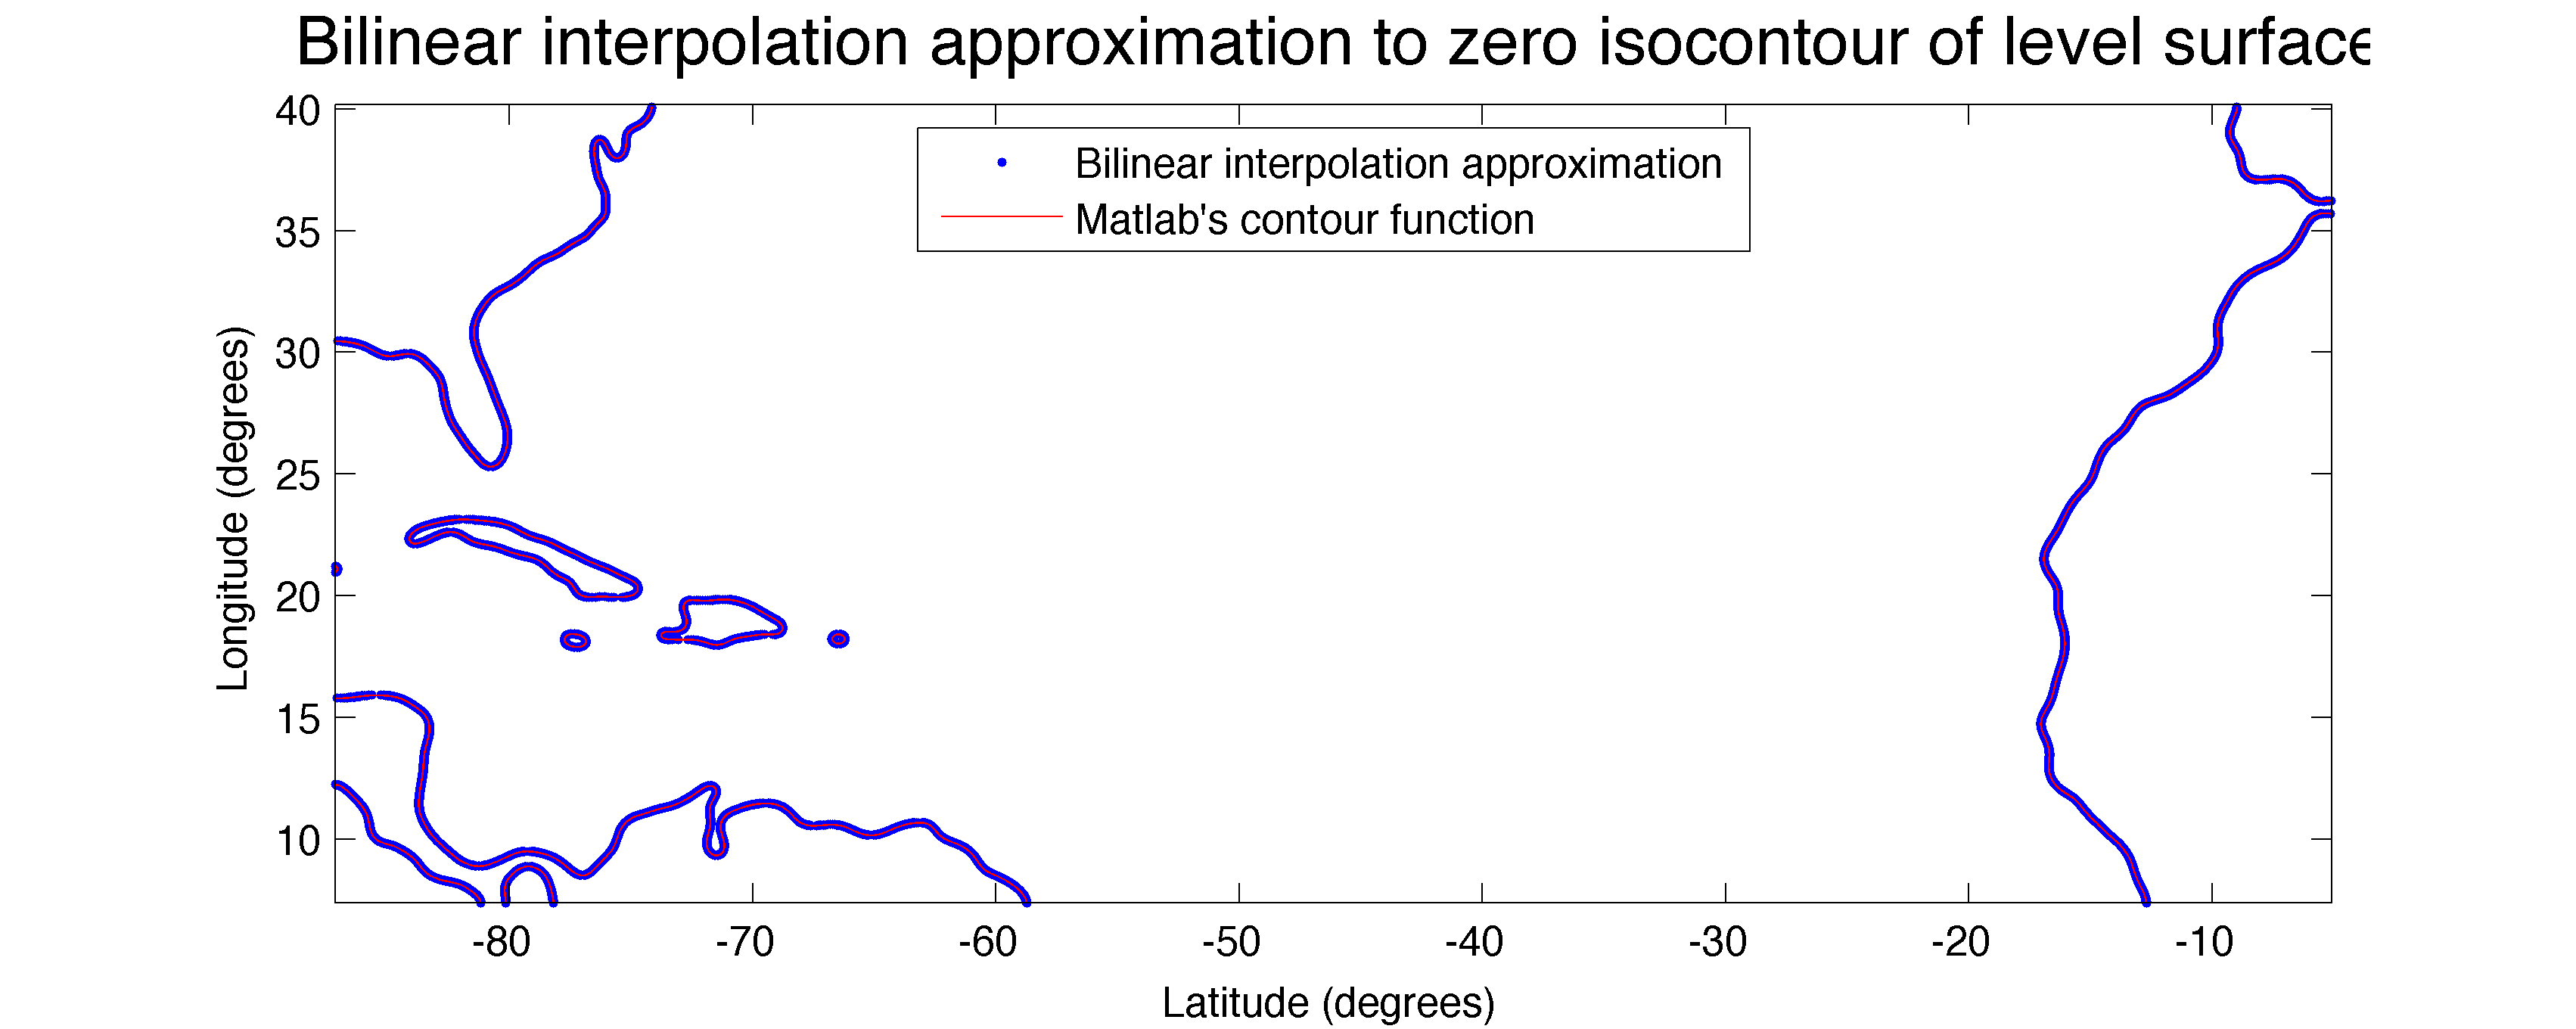
\includegraphics[width=\textwidth]{figures/bilin-interp-approx.png}
  \caption{A plot of the bilinear interpolation approximation to the
zero isocontour of a level surface (blue points). The data used to generate this
image came from
\texttt{constCurv/resdata/mapL\_curvatureLS.tMax2.3.b0.04.mat}. The
red line was computed by \textsc{Matlab}'s \texttt{contour}
function. }
\label{fig:bilin-interp}
\end{figure}

\lstinputlisting[language=matlab]{./../ZCzoom/bilinZC_example.m}

% \subsection{Random Paragraph}
% \label{sec:random-paragraph}

% It is sometimes important to have a irregular representation of
% the coastline. One such way to accomplish this is to obtain a list
% of points $(x,y)$ that are located on the zero isocontour of the
% level surface. To determine such a set of points, we used inverse
% bilinear interpolation to determine up to a fixed number $N$ of
% points in the domain whose image under $\phi$ is zero. That is,
% given an implicit representation of a function
% $\left(\mathbf{F}\right)_{ij}$ on a regular grid, one can
% determine the zero isocontour through a fixed box $[j, j+1] \times
% [i, i+1]$ by 
\clearpage
\bibliographystyle{acm}
\bibliography{bib_evoLS}
\end{document}

%%% Local Variables: 
%%% mode: latex
%%% TeX-master: t
%%% End: 
